\documentclass[tikz,border=8pt]{standalone}
\usepackage{ctex}
\usepackage{amsmath,amssymb}
\usetikzlibrary{arrows.meta,calc,angles,quotes,positioning,decorations.pathmorphing,patterns,3d}
\definecolor{ink}{RGB}{31,43,57}
\definecolor{blue}{RGB}{35,91,166}
\definecolor{orange}{RGB}{224,111,20}
\definecolor{green}{RGB}{35,139,92}
\definecolor{red}{RGB}{190,52,52}
\tikzset{
 line cap=round,line join=round,
 body/.style={draw=ink,very thick},
 axis/.style={-{Latex[length=2.5mm]},draw=ink,very thick},
 vec/.style={-{Latex[length=2.5mm]},draw=blue,very thick},
 force/.style={-{Latex[length=2.5mm]},draw=red,very thick},
 ray/.style={-{Latex[length=2.2mm]},draw=orange,very thick},
 guide/.style={draw=ink!45,dashed},
 dim/.style={{Latex[length=2mm]}-{Latex[length=2mm]},draw=ink!70}
}
\begin{document}

% question-01
\begin{tikzpicture}[scale=.95]
 \draw[body] (-4.6,0)--(4.8,0);
 \foreach \x in {-4.4,-4.0,...,4.6}{\draw[ink!35] (\x,0)--++(-.18,-.18);}
 \foreach \s in {-3.9,-1.3,1.3}{
   \draw[orange,very thick] (\s,0) .. controls +(0.7,1.65) and +(-.7,1.65) .. +(2.35,0);
 }
 \fill[blue] (-3.9,0) circle(3pt);
 \draw[vec] (-3.9,0)--++(1.15,0) node[below] {$u_x$};
 \draw[vec] (-3.9,0)--++(0,1.15) node[left] {$u_y$};
 \draw[force] (-2.15,.85)--++(-.9,0) node[above] {$-k\boldsymbol v$};
 \node[align=center] at (.2,-.85) {稳定周期跳跃：每次起跳状态相同};
\end{tikzpicture}

% solution-01
\begin{tikzpicture}[scale=.9]
 \draw[body] (-4.2,0)--(4.2,0);
 \draw[orange,very thick] (-3.1,0) .. controls +(.9,2.3) and +(-1.0,2.0) .. (2.8,0);
 \fill[ink] (-3.1,0) circle(3pt) node[below] {起跳};
 \fill[ink] (2.8,0) circle(3pt) node[below] {着地前};
 \draw[vec] (-3.1,0)--++(1.15,0) node[below] {$u_x$};
 \draw[vec] (-3.1,0)--++(0,1.25) node[left] {$u_y$};
 \draw[vec] (2.8,0)--++(.75,0) node[below] {$u'_x$};
 \draw[vec] (2.8,0)--++(0,-1.1) node[right] {$u'_y<0$};
 \draw[force] (3.6,-1.35)--++(-1.0,0) node[below] {$I_f$};
 \draw[force] (3.6,-1.35)--++(0,1.15) node[right] {$I_N$};
 \draw[dim] (-3.1,-1.65)--(2.8,-1.65) node[midway,below] {$\Delta x$};
 \node[draw=ink!35,rounded corners,fill=white] at (0,2.55)
 {$I_f\leq\mu I_N$，极值时取等号};
\end{tikzpicture}

% question-02
\begin{tikzpicture}[scale=.95]
 \coordinate (A) at (-2.2,1.75); \coordinate (B) at (2.2,1.75); \coordinate (C) at (0,-2.05);
 \fill[orange!10] (A)--(B)--(C)--cycle;
 \draw[body] (A)--(B)--(C)--cycle;
 \fill[ink] (0,.48) circle(3pt) node[right] {$G$};
 \draw[body,line width=3pt] (C)--++(0,-.55);
 \fill[blue] (-3.2,-2.05) circle(5pt) node[below] {$m$};
 \draw[vec] (-3.2,-2.05)--++(1.35,0) node[below] {$v_0$};
 \draw[dim] (-2.2,2.2)--(2.2,2.2) node[midway,above] {$a$};
 \node at (0,-3.1) {小球与三角板顶点处轻质挡板完全弹性碰撞};
\end{tikzpicture}

% solution-02
\begin{tikzpicture}[scale=.82]
 \begin{scope}[xshift=-4.5cm]
  \coordinate (A) at (-1.4,1.2); \coordinate (B) at (1.4,1.2); \coordinate (C) at (0,-1.25);
  \draw[body] (A)--(B)--(C)--cycle; \fill[orange] (0,.38) circle(3pt) node[right] {$G$};
  \fill[blue] (-2.25,-1.25) circle(4pt);
  \draw[vec] (-2.25,-1.25)--++(1.05,0) node[below] {$v_0$};
  \draw[force] (C)--++(1.2,0) node[below] {$J$};
  \draw[dim] (.28,-1.25)--(.28,.38) node[midway,right] {$a/\sqrt3$};
  \node at (0,-2.2) {第一次碰撞};
 \end{scope}
 \begin{scope}[xshift=3.6cm]
  \coordinate (A) at (-1.4,1.2); \coordinate (B) at (1.4,1.2); \coordinate (C) at (0,-1.25);
  \draw[body] (A)--(B)--(C)--cycle; \fill[orange] (0,.38) circle(3pt);
  \draw[vec] (0,.38)--++(1.0,0) node[above] {$u_1$};
  \draw[vec] (.55,.25) arc[start angle=-25,end angle=275,radius=.55] node[right] {$\omega_1$};
  \fill[blue] (-1.8,-1.25) circle(4pt); \draw[vec] (-1.8,-1.25)--++(.8,0) node[below] {$v_1$};
  \node[align=center] at (0,-2.25) {$m/M=1/3$ 时\\下一顶点可再次相碰};
 \end{scope}
\end{tikzpicture}

% question-03
\begin{tikzpicture}[scale=.9]
 \foreach \x/\lab/\rad in {-4.8/1/.30,-2.4/2/.38,0/3/.46,2.4/4/.54,4.8/5/.62}{
  \draw[body,fill=blue!8] (\x,0) circle(\rad);
  \node at (\x,1.05) {$N=\lab$};
 }
 \node at (-4.8,-1.05) {$V_1(1)=2$};
 \node at (-2.4,-1.05) {$V_2(1)=\pi$};
 \node at (0,-1.05) {$V_3(1)=\dfrac{4\pi}{3}$};
 \node at (2.4,-1.05) {$V_4(1)=\dfrac{\pi^2}{2}$};
 \node at (4.8,-1.05) {$V_5(1)=\dfrac{8\pi^2}{15}$};
 \draw[guide] (-5.6,-1.55)--(5.6,-1.55);
 \node at (0,-2.1) {单位 $N$ 维球的体积系数};
\end{tikzpicture}

% solution-03
\begin{tikzpicture}[scale=.9]
 \draw[body,fill=blue!7] (0,0) circle(2.2);
 \draw[body,fill=white] (0,0) circle(1.55);
 \draw[dim] (0,0)--(2.2,0) node[midway,above] {$r$};
 \draw[force] (2.2,0)--++(.8,0) node[right] {$p_{\rm in}-p_{\rm out}$};
 \draw[green,very thick] (0,2.2) arc[start angle=90,end angle=15,radius=2.2];
 \node[green] at (1.45,1.85) {$\sigma_N\,dS_N$};
 \begin{scope}[xshift=5cm]
  \draw[body,fill=orange!8] (-1.1,-2)--(1.1,-2)--(1.1,2)--(-1.1,2)--cycle;
  \draw[body] (0,2) ellipse(1.1 and .35); \draw[body] (0,-2) ellipse(1.1 and .35);
  \draw[dim] (0,-2.55)--(0,2.55) node[midway,right] {$L$};
  \draw[dim] (0,0)--(1.1,0) node[midway,above] {$r$};
  \node at (0,-3.1) {$N$ 维液柱：一个方向平移对称};
 \end{scope}
\end{tikzpicture}

% question-04
\begin{tikzpicture}[scale=.9]
 \foreach \k in {0,...,5}{\coordinate (P\k) at ({90-60*\k}:2.0);}
 \fill[blue!8] (P0)--(P1)--(P2)--(P3)--(P4)--(P5)--cycle;
 \draw[body] (P0)--(P1)--(P2)--(P3)--(P4)--(P5)--cycle;
 \draw[ray] (-4,.45)--(-1.72,.45)--(.9,-.35)--(3.7,-.9);
 \draw[guide] (-1.72,.45)--++(150:1.2); \draw[guide] (.9,-.35)--++(30:1.2);
 \node[blue] at (-2.15,.95) {$\alpha$};
 \node[orange] at (2.1,-.25) {$\theta$};
 \node at (0,-2.85) {六角冰晶截面中的两次折射};
\end{tikzpicture}

% solution-04
\begin{tikzpicture}[scale=.82]
 \begin{scope}[xshift=-4.0cm]
  \draw[body] (-1.7,1.4)--(0,0)--(1.7,1.4);
  \draw[guide] (0,0)--(0,2.2);
  \draw[ray] (-2.6,.2)--(0,0)--(2.6,.2);
  \draw[blue] (0,.75) arc[start angle=90,end angle=130,radius=.75];
  \node[blue] at (-.55,.85) {$\beta_1=\pi/6$};
  \node[align=center] at (0,-1.0) {最小偏向时\\光路关于棱镜对称};
 \end{scope}
 \begin{scope}[xshift=3.9cm]
  \draw[body,line width=3pt] (0,-1.6)--(0,1.6) node[above] {镜头，直径 $D$};
  \draw[body] (2.7,-1.7)--(2.7,1.7) node[above] {底片};
  \draw[ray] (-3,1.0)--(0,.6)--(1.7,0)--(2.7,.35);
  \draw[ray] (-3,-1.0)--(0,-.6)--(1.7,0)--(2.7,-.35);
  \fill[ink] (1.7,0) circle(3pt) node[below] {$f$};
  \draw[dim] (2.7,-.35)--(2.7,.35) node[midway,right] {弥散斑};
  \node at (0,-2.25) {相机对焦近处人物时，太阳像落在底片之前};
 \end{scope}
\end{tikzpicture}

% question-05
\begin{tikzpicture}[scale=.92]
 \coordinate (A) at (-2.7,-1.55); \coordinate (B) at (2.7,-1.35); \coordinate (C) at (-.15,2.45); \coordinate (D) at (.75,-.05);
 \fill[blue!6] (A)--(B)--(C)--cycle;
 \draw[body] (A)--(B)--(C)--cycle;
 \draw[ink!70,very thick,densely dashed] (D)--(A) (D)--(B) (D)--(C);
 \foreach \p/\lab in {A/1,B/2,C/3}{\fill[ink] (\p) circle(3pt) node[above right] {$\lab$};}
 \fill[white] (D) circle(5pt); \draw[ink,very thick] (D) circle(5pt);
 \node[above right=1pt] at (D) {$0$};
 \node[fill=white] at (0,-1.45) {$R$};
 \node[fill=white,rotate=55] at (-1.35,.45) {$C$};
 \node[fill=white,rotate=-51] at (1.35,.55) {$L$};
 \node[fill=white,rotate=-24] at (-1.0,-.78) {$L$};
 \node[fill=white,rotate=19] at (1.72,-.65) {$C$};
 \node[fill=white,rotate=-22] at (.28,1.18) {$R$};
 \draw[vec] (-2.7,-2.25)--++(0,1) node[left] {$I$};
 \draw[vec] (2.7,-.35)--++(0,-1) node[right] {$I$};
 \node at (0,-2.85) {正四面体透视图；虚线连接背面顶点 $0$};
\end{tikzpicture}

% solution-05
\begin{tikzpicture}[scale=.9]
 \node[circle,draw=ink,very thick] (n1) at (-3,0) {$1$};
 \node[circle,draw=ink,very thick] (n2) at (3,0) {$2$};
 \node[circle,draw=ink,very thick] (n3) at (0,1.8) {$3$};
 \node[circle,draw=ink,very thick] (n0) at (0,-1.8) {$0$};
 \draw[body] (n1)--node[above] {$R$}(n2);
 \draw[body] (n1)--node[above left] {$-iR$}(n3);
 \draw[body] (n3)--node[above right] {$iR$}(n2);
 \draw[body] (n1)--node[below left] {$iR$}(n0);
 \draw[body] (n0)--node[below right] {$-iR$}(n2);
 \draw[body] (n3)--node[right] {$R$}(n0);
 \node[draw=ink!35,rounded corners,fill=white] at (0,-3.0)
 {$V_3-V_0=i(V_1-V_2)$，故 $Z_{\rm eq}=R/2$};
\end{tikzpicture}

% question-06
\begin{tikzpicture}[scale=.9]
 \shade[ball color=blue!25] (-4.3,0) circle(1.35); \draw[body] (-4.3,0) circle(1.35); \node at (-4.55,-.2) {$A,Z$};
 \draw[axis] (-2.6,0)--(-1.1,0);
 \shade[ball color=orange!28] (.15,.8) circle(.95); \draw[body] (.15,.8) circle(.95);
 \shade[ball color=orange!28] (.15,-1.0) circle(.75); \draw[body] (.15,-1.0) circle(.75);
 \node at (-.05,.55) {$A_1,Z_1$}; \node at (-.10,-.78) {$A_2,Z_2$};
 \draw[axis] (1.35,0)--(2.7,0);
 \shade[ball color=orange!28] (4.1,.9) circle(.95); \draw[body] (4.1,.9) circle(.95);
 \shade[ball color=orange!28] (4.1,-1.25) circle(.75); \draw[body] (4.1,-1.25) circle(.75);
 \draw[guide] (4.1,-.05)--(4.1,-.5);
 \draw[dim] (-4.3,0)--(-3.45,.85) node[midway,above left] {$R_0$};
 \draw[dim] (.15,.8)--(.82,1.47) node[midway,above right] {$R_1$};
 \draw[dim] (.15,-1.0)--(.68,-1.53) node[midway,below right] {$R_2$};
 \node[align=center] at (-4.3,-2.05) {母核};
 \node[align=center] at (.15,-2.05) {刚接触的两个子核};
 \node[align=center] at (4.1,-2.35) {相距很远的子核};
\end{tikzpicture}

% solution-06
\begin{tikzpicture}[scale=.88]
 \begin{scope}[xshift=-5.2cm]
  \shade[ball color=blue!25] (0,.2) circle(1.22); \draw[body] (0,.2) circle(1.22);
  \draw[dim] (0,.2)--(1.22,.2) node[midway,above] {$R_0$};
  \node at (0,-1.55) {$U_{\rm S0},\ U_{\rm E0}$};
  \node at (0,-2.05) {母核};
 \end{scope}
 \draw[axis] (-3.7,.2)--(-2.6,.2);
 \begin{scope}
  \shade[ball color=orange!28] (0,.98) circle(.88); \draw[body] (0,.98) circle(.88);
  \shade[ball color=orange!28] (0,-.58) circle(.68); \draw[body] (0,-.58) circle(.68);
  \draw[dim] (0,.98)--(.88,.98) node[midway,above] {$R_1$};
  \draw[dim] (0,-.58)--(.68,-.58) node[midway,below] {$R_2$};
  \node at (0,-1.65) {$\alpha U_{\rm S0},\ \beta U_{\rm E0}$};
  \node at (0,-2.15) {刚相切};
 \end{scope}
 \draw[axis] (1.55,.2)--(2.65,.2);
 \begin{scope}[xshift=5.2cm]
  \shade[ball color=orange!28] (0,1.25) circle(.88); \draw[body] (0,1.25) circle(.88);
  \shade[ball color=orange!28] (0,-1.0) circle(.68); \draw[body] (0,-1.0) circle(.68);
  \node at (0,-2.0) {$\alpha U_{\rm S0},\ \gamma U_{\rm E0}$};
  \node at (0,-2.5) {相距无穷远};
 \end{scope}
 \draw[dim] (-4.2,2.45)--(4.2,2.45) node[midway,above] {终态相对初态释放能量 $Q$};
\end{tikzpicture}

% question-07
\begin{tikzpicture}[scale=.95]
 \draw[body,fill=blue!6] (-3.0,-.1) arc[start angle=210,end angle=-25,radius=3.0];
 \draw[force] (-2.6,-1.5)--++(-1.2,-.4) node[left] {$J$};
 \draw[vec] (2.7,-1.3)--++(.9,-.3) node[right] {$v$};
 \draw[blue] (0,0)++(210:1.1) arc[start angle=210,end angle=335,radius=1.1];
 \node[blue] at (0,-1.45) {$\Theta$};
 \node at (0,-3.6) {不可伸长均匀细绳形成圆弧，端点受切向冲量};
\end{tikzpicture}

% solution-07
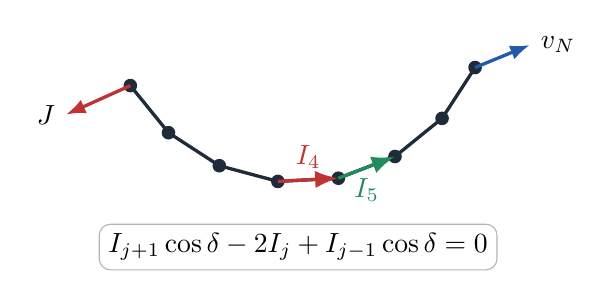
\begin{tikzpicture}[scale=.82]
 \foreach \j in {0,...,7}{
  \coordinate (P\j) at ({210+18*\j}:3.0);
  \fill[ink] (P\j) circle(3pt);
 }
 \foreach \j in {0,...,6}{\pgfmathtruncatemacro{\k}{\j+1}\draw[body] (P\j)--(P\k);}
 \draw[force] (P0)--++(-1.0,-.45) node[left] {$J$};
 \draw[vec] (P7)--++(.85,.35) node[right] {$v_N$};
 \draw[red,very thick,-{Latex}] (P3)--(P4) node[midway,above] {$I_4$};
 \draw[green,very thick,-{Latex}] (P4)--(P5) node[midway,below] {$I_5$};
 \node[draw=ink!35,rounded corners,fill=white] at (0,-4.0)
 {$I_{j+1}\cos\delta-2I_j+I_{j-1}\cos\delta=0$};
\end{tikzpicture}

% question-08
\begin{tikzpicture}[scale=.9]
 \shade[ball color=blue!18,opacity=.55] (0,0) circle(2.2);
 \draw[body] (0,0) circle(2.2);
 \draw[guide] (-2.2,0) arc[start angle=180,end angle=360,x radius=2.2,y radius=.65];
 \draw[ink!55,densely dashed] (2.2,0) arc[start angle=0,end angle=180,x radius=2.2,y radius=.65];
 \draw[axis] (0,0)--(3.0,0) node[right] {$p_x$};
 \draw[axis] (0,0)--(0,3.0) node[above] {$p_y$};
 \draw[axis] (0,0)--(-1.8,-1.8) node[below left] {$p_z$};
 \draw[dim] (0,0)--(1.55,1.55) node[midway,above left] {$p$};
 \draw[orange,very thick] (0,0) circle(1.55);
 \draw[orange!70,densely dashed] (-1.55,0) arc[start angle=180,end angle=360,x radius=1.55,y radius=.46];
 \node[orange] at (2.0,1.7) {$4\pi p^2\,dp$};
 \node at (0,-3.05) {各向同性动量分布的球壳};
\end{tikzpicture}

% solution-08
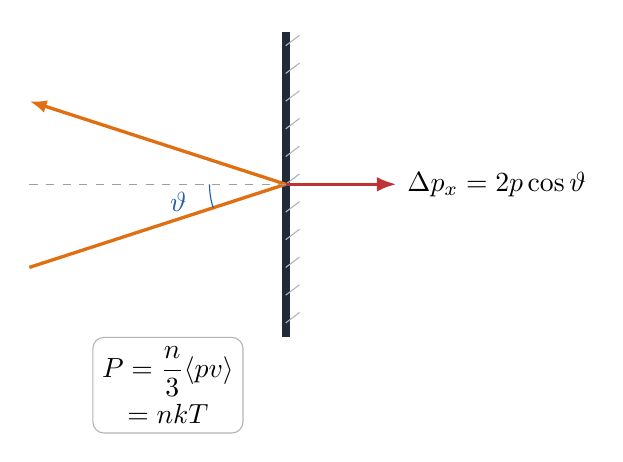
\begin{tikzpicture}[scale=.88]
 \draw[body,line width=3pt] (0,-2.2)--(0,2.2);
 \foreach \y in {-2,-1.6,...,2}{\draw[ink!35] (0,\y)--++(.2,.15);}
 \draw[ray] (-3.7,-1.2)--(0,0)--(-3.7,1.2);
 \draw[guide] (-3.7,0)--(.7,0);
 \draw[blue] (-1.1,0) arc[start angle=180,end angle=198,radius=1.1];
 \node[blue] at (-1.55,-.25) {$\vartheta$};
 \draw[force] (0,0)--++(1.6,0) node[right] {$\Delta p_x=2p\cos\vartheta$};
 \node[draw=ink!35,rounded corners,fill=white,align=center] at (-1.7,-2.9)
 {$P=\dfrac n3\langle p v\rangle$\\[2pt]$=nkT$};
\end{tikzpicture}

\end{document}
